%-----------------------------------------------------
% Chapter: Introduction
%-----------------------------------------------------
\chapter{Introduction}
\label{chap:intro}
\section{Overview}
Natural language is a constantly evolving system capable of  producing infinite numbers of sentences each with their own distinct meaning. Even from a young age, the task of inferring meaning from a sentence is one that is seemingly trivial for humans. However, getting machines to derive meaning from textual data has long been a challenge within the field of Artificial Intelligence, specifically the subfield of Natural Language Processing (NLP). Representing words as numerical data, also known as word embeddings, is the first step in bridging the gap between natural language and machines. Previous methods to create such representations include the one-hot encoding method which involves encoding words as word vectors which have as many dimensions as the number of unique words within a corpora. Each dimension in the vector is assigned a zero value except for the dimension representing the word which is assigned a value of 1.

\noindent
\newline
The resulting word embeddings obtained from these types of methods are sparse and suffer from the curse of dimensionality due to the dimensionality of the word vector growing linearly with the size of the vocabulary. Moreover, these representations fail to capture any syntactic and semantic relationships contained within textual data. Recent word embedding methods rely on the intuition that word meaning can be inferred from context. Specifically, these methods are based on the distributional hypothesis (\cite{Harris1954}) that states that words which appear in a similar context have similar meanings. Algorithms such as GloVe (\cite{Pennington2014}) and word2vec (\cite{Mikolov2013}) exploit this concept to produce dense real valued word embeddings, which are able to encode syntactic and semantic regularities.

\noindent
\newline
Language Modelling and Text Classification are two active research areas in NLP which have benefited greatly from dense word embeddings. The usage of these word embeddings has helped improve accuracy in tasks such as Document Classification and Named-Entity Recognition. State of the art results in both areas have utilised recurrent neural networks which utilise word embeddings within an embedding layer to convert text corpora into inputs for the network.

\noindent
\newline
Often accompanying text corpora are associated covariates, e.g. author demographic or publication genre, which provide additional metadata about a corpus. CoVeR (\cite{Tian2018}), a novel tensor decomposition method for learning covariate specific word embeddings, is an extension of the GloVe algorithm which aims to encode covariate information with learned embeddings.

\section{The Songwriters Dilemma}
Songwriting is an integral part of the song making process which often draws upon past events and experiences. Structure and content both contribute heavily towards the success of a song; with the latter being a key factor on the extent to which a song resonates with a listener. A problem commonly faced by songwriters is that of word choice, through which they can express their ideas clearly and concisely.

\noindent
\newline
In general, skilled writers are attributed with having vast vocabulary ranges. For adults, the average vocabulary ranges between 15,000-23,000 words (\cite{McCrum2011}). Examining his works alone, Shakespeare is said to have had an approximate vocabulary range of 30,000-65,000 words\footnote{https://kottke.org/10/04/how-many-words-did-shakespeare-know} \footnote{This range is most likely skewed as variant forms of words are included as singular counts}. Nonetheless, a skilled songwriters ability to write impactful lyrics is not down to vocabulary size alone, but effective word choice.
 
\noindent
\newline
As shown in a study examining vocabulary range within Hip-Hop\footnote{https://pudding.cool/projects/vocabulary/index.html}, which recently surpassed Rock as the most popular genre in America\footnote{https://www.nielsen.com/us/en/insights/reports/2018/2017-music-us-year-end-report.html}, more is not always better. The study examines the unique word count of 150 famous Hip-Hop artists across their first 35,000 lyrics. Aesop Rock, ranked 1st on the list, recorded a count of 7,392 unique words across his first 35,000 lyrics. In contrast, rappers Drake and Future, ranked 130th and 131st respectively, had an average unique word count of 3,334 words used across their first 35,000 lyrics; a 55\% decrease from Aesop Rocks count. 
\begin{figure}[h]	
	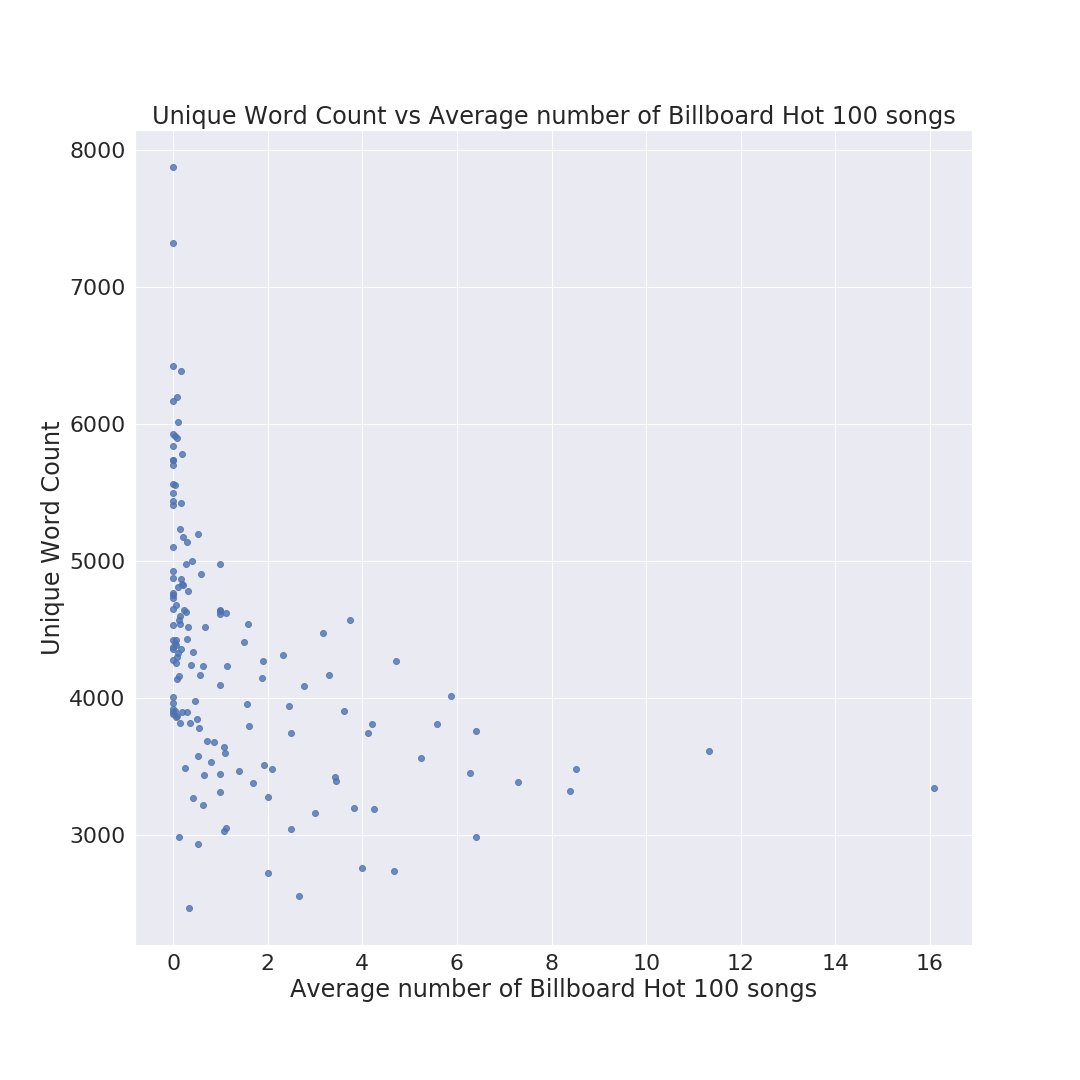
\includegraphics[width=10cm, height=10cm]{./figures/fig1}
	\centering
	\caption{Average number of Billboard 100 songs during artist activity, compared to unique word count across an artists first 35,000 words.}
	\label{fig:fig1}
\end{figure}

\noindent
\newline
To validate the earlier claim that vocabulary range is not indicative of a songwriters ability to write impactful lyrics, the unique word count per artist was compared against the average number of Billboard 100\footnote{https://www.billboard.com/charts/hot-100} songs across an artist had across their career. Pearson's Correlation Coefficient , which is used to measure the linear relationship between two variables, was applied to both unique word count and average number of Billboard 100 songs. This resulted in a correlation coefficient of -0.42, indicating a weak inverse correlation between the pairs of data. This value supports the earlier claim that vocabulary range is not indicative of a songwriters ability.

\noindent
\newline
Common methods used to improve songwriting competency include group writing and vocabulary expansion. More recently, software solutions such as MasterWriter\footnote{https://masterwriter.com/5} have been used to consolidate previous methods. An inherent problem within software solutions like MasterWriter is the static nature of features such as fixed word and rhyming dictionaries. Consequently, these applications fail to address the ambiguous usage of words resulting from the emerging nature of natural language.

\noindent
\newline
After the completion of song lyrics another secondary problem often faced by less experienced songwriters is choice of instrumental style. 

\section{Aims and Objectives}
The aim of this project is to explore the use of covariate specific word embeddings within both  language modelling and text classification tasks. To contextualise the project aims, both models are applied to a possible use case: a prototype software solution to help reduce common problems faced by songwriters, namely:

\begin{enumerate}
	\item Word Choice 
	\item Lyric classification
\end{enumerate}

\noindent
\newline
With this in mind, a prototype solution, SONGIFAI is proposed. SONGIFAI provides two main features namely lyric assistance through predictive text and a word suggestion feature, as well as genre classification for a given lyric. The covariates explored in this project are the following music genres: \textit{Pop}, \textit{Rock} and \textit{Hip-Hop}. 

\noindent
\newline
As stated before, recurrent neural networks have been used successfully in both language modelling and text classification tasks. The specific variant of the recurrent neural network which has been successfully utilised in these tasks is the Long Short-Term Memory network (discussed in more detail \autoref{chap:background}). This network architecture is used for both the language model and text classifier which are utilised for the word prediction and lyric classification features respectively. The word suggestion feature utilises the covariate specific embeddings themselves. A high level system architecture of the prototype can be seen in \autoref{fig:fig7}5
\begin{figure}[h]	
	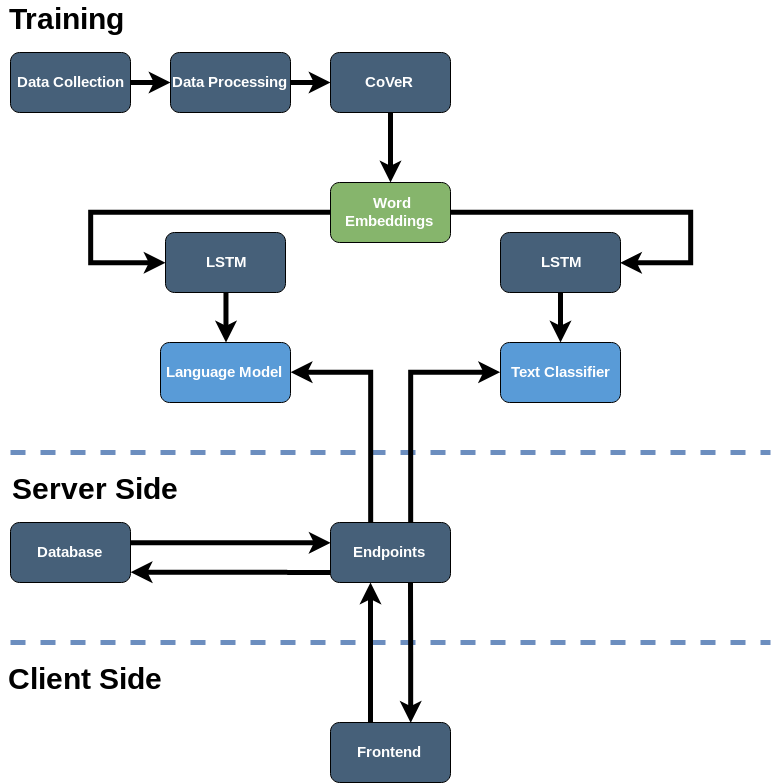
\includegraphics[width=13cm, height=14cm]{./figures/fig7}
	\centering
	\caption{High level system architecture for the prototype which takes the form of a full software system}
	\label{fig:fig7}
\end{figure}
